\subsection{Cadre du TER}
\begin{frame}{Cadre et objectifs}
	\begin{itemize}
		\item Ce TER se situe dans le cadre de Problème de flot maximum

		\item Il existe différents types d'algorithmes répondant à ce problème, certains basés sur la recherche
			de chaînes améliorantes (Edmonds-Karp, Ford Fulkerson, ...), d'autres sur les fonctions de préflots. 
			Nous nous intéresserons à la seconde catégorie.
	\end{itemize}
\end{frame}

\subsection{Motivation}
\begin{frame}{Utilité}
	
	Considérons une entreprise, devant acheminer sa production depuis
	l'usine de création au lieu de stockage. \vfill

	\begin{center}
		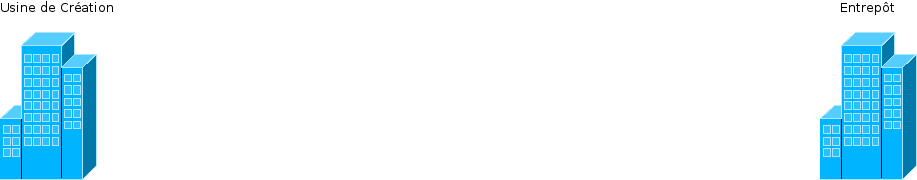
\includegraphics[scale=0.32]{img/etape1.png}
	\end{center}
\end{frame}

\begin{frame}{Utilité}
	Il existe différents points, par lesquels peut transiter la production.

	\begin{center}
		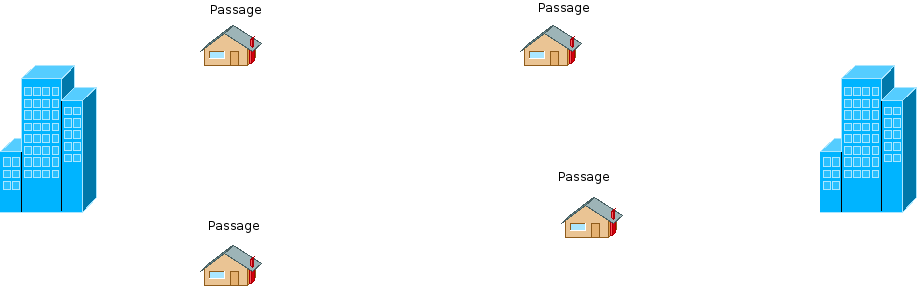
\includegraphics[scale=0.32]{img/etape2.png}
	\end{center}
\end{frame}

\begin{frame}{Utilité}
	Chaque passage est reliés aux autres à l'aide de routes permettant un transit plus ou moins facile
	jusqu'à destination.

	\begin{center}
		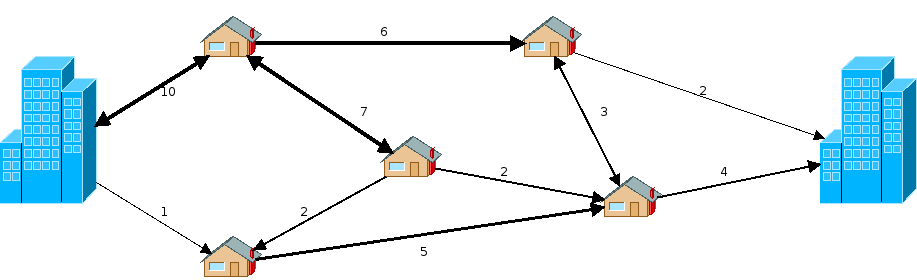
\includegraphics[scale=0.32]{img/exemple.png}
	\end{center}
\end{frame}

\begin{frame}{Utilité}
	Chaque passage est reliés aux autres à l'aide de routes permettant un transit plus ou moins facile
	jusqu'à destination.

	\begin{center}
		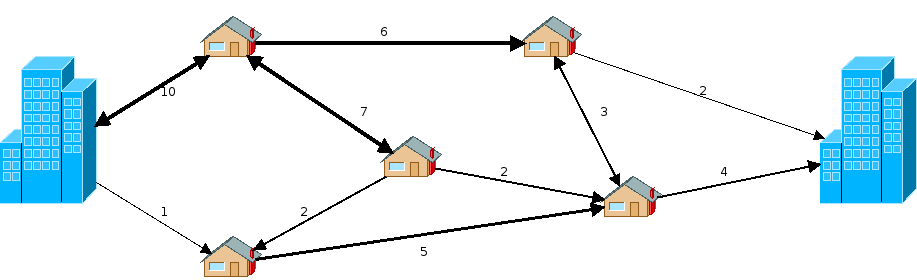
\includegraphics[scale=0.32]{img/exemple.png}
	\end{center}

	\begin{alertblock}{Bingo!}
		Il s'agit là d'un problème de flot maximum.
	\end{alertblock}
\end{frame}

\subsection{Les algorithmes de chaînes améliorantes}
\begin{frame}{Définitions}
		Nous allons définir quelques notions qui seront utlisées par la suite
		pour le déroulement de l'algorithme de préflot et ses dérivés.
\end{frame}

\begin{frame}{La notion de flot}
	Un flot est une fonction de graphes vérifiant certaines propriétés, qui sont : \vfill \vfill
\end{frame} 

\begin{frame}{La notion de flot}
	Un flot est une fonction de graphes vérifiant certaines propriétés, qui sont : ~\\~\\
	\begin{exampleblock}{le respect de la capacité de l'arc}
		La valeur du flot sur un arc ne peut être supérieure à la capacité de l'arc et ne peut être négative
	\end{exampleblock}\vfill
\end{frame} 

\begin{frame}{La notion de flot}
	Un flot est une fonction de graphes vérifiant certaines propriétés, qui sont :~\\~\\
	\begin{block}{le respect de la capacité de l'arc}
		$$\forall (i,j) \in A, \quad 0 \leq x(i,j) \leq c(i,j)$$
	\end{block}\vfill
	\begin{exampleblock}{le respect de la loi de Kirchoff}
		Pour chaque noeud différent de la source et du puits, la quantité de flot entrant dans le noeud
		est égale à la quantité de flot sortant de ce dernier.
	\end{exampleblock}\vfill
\end{frame} 

\begin{frame}{La notion de flot}
	Un flot est une fonction de graphes vérifiant certaines propriétés, qui sont : 
	\begin{block}{le respect de la capacité de l'arc}
		$$\forall (i,j) \in A, \quad 0 \leq x(i,j) \leq c(i,j)$$
	\end{block}\vfill
	\begin{block}{le respect de la loi de Kirchoff}
		$$\forall i \in S - \{s,t\}, \quad \sum_{j \in A^+(i)} x(i,j) = \sum_{k\in A^-(i)} x(k,i)$$
	\end{block}\vfill
	\begin{exampleblock}{Le respect de la contrainte de symétrie}
		Pour chaque arc du graphe, il n'y a aucun phénomène de perte entre le sommet de départ et le
		sommet d'arrivée.
	\end{exampleblock}\vfill
\end{frame} 

\begin{frame}{La notion de flot}
	Un flot est une fonction de graphes vérifiant certaines propriétés, qui sont : 
	\begin{block}{le respect de la capacité de l'arc}
		$$\forall (i,j) \in A, \quad 0 \leq x(i,j) \leq c(i,j)$$
	\end{block}\vfill
	\begin{block}{le respect de la loi de Kirchoff}
		$$\forall i \in S - \{s,t\}, \quad \sum_{j \in A^+(i)} x(i,j) = \sum_{k\in A^-(i)} x(k,i)$$
	\end{block}\vfill
	\begin{block}{Le respect de la contrainte de symétrie}
		$$ f = \sum_{j \in A^+(s)} x(s,j) = \sum_{k\in A^- (t)} x(k,t) $$ 
	\end{block}\vfill
\end{frame} 

\begin{frame}{Le réseau résiduel}
 	Soit un graphe $G(S, A)$, un flot $f$ et $i,j$ deux sommets de $G$. On dira que
	l'arête $(i,j)$ appartiendra au réseau résiduel $A_f$ si et seulement si la capacité résiduelle
	est non nulle.

	\begin{alertblock}{Autrement dit}
	 	$$ r(i,j) = c(i,j) - x(i,j) > 0 $$ 
	\end{alertblock}

	On appelle alors $r(i,j)$ la capacité résiduelle de l'arête $(i,j)$. 
	\vfill
\end{frame}

\begin{frame}{Le réseau résiduel}
 	Soit un graphe $G(S, A)$, un flot $f$ et $i,j$ deux sommets de $G$. On dira que
	l'arête $(i,j)$ appartiendra au réseau résiduel $A_f$ si et seulement si la capacité résiduelle
	est non nulle.

	\begin{alertblock}{Autrement dit}
	 	$$ r(i,j) = c(i,j) - x(i,j) > 0 $$ 
	\end{alertblock}


	On appelle alors $r(i,j)$ la capacité résiduelle de l'arête $(i,j)$. 

	\begin{block}{Note}
		Si $x(i,j) > 0$ alors $(j,i)$ appartient au réseau résiduel avec une capacité résiduelle $r(j,i) = x(i,j)$.
	\end{block}
\end{frame}

\begin{frame}{Le réseau résiduel}
 	Soit un graphe $G(S, A)$, un flot $f$ et $i,j$ deux sommets de $G$. On dira que
	l'arête $(i,j)$ appartiendra au réseau résiduel $A_f$ si et seulement si la capacité résiduelle
	est non nulle.

	\begin{alertblock}{Autrement dit}
	 	$$ r(i,j) = c(i,j) - x(i,j) > 0 $$ 
	\end{alertblock}


	On appelle alors $r(i,j)$ la capacité résiduelle de l'arête $(i,j)$. 

	\begin{alertblock}{Théorème}
	S'il existe un chemin de la source au puits dans le réseau résiduel, alors on peut augmenter la
	valeur du flot dans le graphe. Ce chemin est appelé chaîne améliorante.
	\end{alertblock}
\end{frame}

\begin{frame}{Le réseau résiduel}
	Pour le flot suivant, ... \vfill
	\begin{minipage}[c]{0.45\linewidth}
		\begin{figure}
			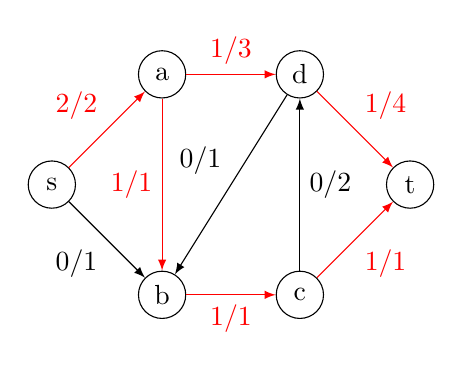
\begin{tikzpicture}[scale=0.7]
				\tikzset{noeud/.style={circle, draw=black, inner sep=0.1cm, minimum width=0.6cm}, fleche/.style={>=latex, ->}};
				\node[noeud] (s) at (0,0) {s};
				\node[noeud] (a) at (2, 2) {a};
				\node[noeud] (b) at (2, -2) {b};
				\node[noeud] (c) at (4.5, -2) {c};
				\node[noeud] (d) at (4.5, 2) {d};
				\node[noeud] (t) at (6.5,0) {t};

				\draw[fleche, red] (s) -- node[above left, red] {$2/2$}(a);
				\draw[fleche] (s) -- node[below left] {$0/1$}(b);
				\draw[fleche, red] (a) -- node[left,red] {$1/1$}(b);
				\draw[fleche, red] (a) -- node[above, red] {$1/3$}(d);
				\draw[fleche] (d) -- node[above left] {$0/1$}(b);
				\draw[fleche, red] (b) -- node[below, red] {$1/1$}(c);
				\draw[fleche, red] (d) -- node[above right, red] {$1/4$}(t);
				\draw[fleche, red] (c) -- node[below right, red] {$1/1$}(t);
				\draw[fleche] (c) -- node[right] {$0/2$}(d);
			\end{tikzpicture}
			\caption{Un exemple de flot}
		\end{figure}
	\end{minipage} \hfill
	\begin{minipage}[c]{0.45\linewidth}
	\end{minipage}
\end{frame}

\begin{frame}{Le réseau résiduel}
	$\dots$ on a le réseau résiduel suivant : \vfill
	\begin{minipage}[c]{0.45\linewidth}
		\begin{figure}
			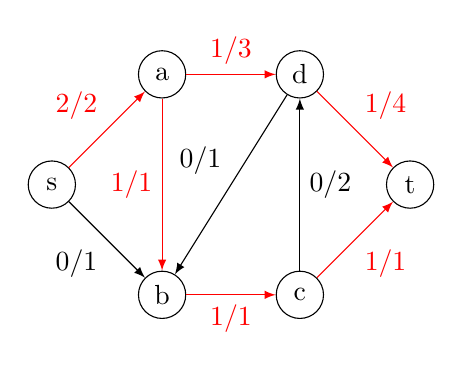
\begin{tikzpicture}[scale=0.7]
				\tikzset{noeud/.style={circle, draw=black, inner sep=0.1cm, minimum width=0.6cm}, fleche/.style={>=latex, ->}};
				\node[noeud] (s) at (0,0) {s};
				\node[noeud] (a) at (2, 2) {a};
				\node[noeud] (b) at (2, -2) {b};
				\node[noeud] (c) at (4.5, -2) {c};
				\node[noeud] (d) at (4.5, 2) {d};
				\node[noeud] (t) at (6.5,0) {t};

				\draw[fleche, red] (s) -- node[above left, red] {$2/2$}(a);
				\draw[fleche] (s) -- node[below left] {$0/1$}(b);
				\draw[fleche, red] (a) -- node[left,red] {$1/1$}(b);
				\draw[fleche, red] (a) -- node[above, red] {$1/3$}(d);
				\draw[fleche] (d) -- node[above left] {$0/1$}(b);
				\draw[fleche, red] (b) -- node[below, red] {$1/1$}(c);
				\draw[fleche, red] (d) -- node[above right, red] {$1/4$}(t);
				\draw[fleche, red] (c) -- node[below right, red] {$1/1$}(t);
				\draw[fleche] (c) -- node[right] {$0/2$}(d);
			\end{tikzpicture}
			\caption{Un exemple de flot}
		\end{figure}
	\end{minipage} \hfill
	\begin{minipage}[c]{0.45\linewidth}
		\begin{figure}
			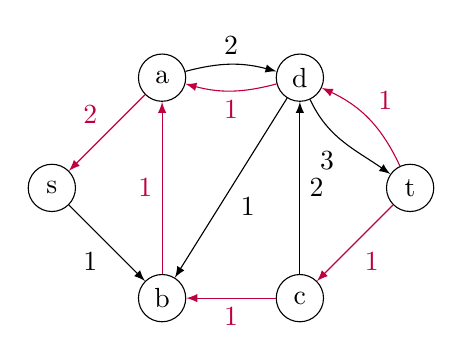
\begin{tikzpicture}[scale=0.7]
				\tikzset{noeud/.style={circle, draw=black, inner sep=0.1cm, minimum width=0.6cm}, fleche/.style={>=latex, ->}};
				\node[noeud] (s) at (0,0) {s};
				\node[noeud] (a) at (2, 2) {a};
				\node[noeud] (b) at (2, -2) {b};
				\node[noeud] (c) at (4.5, -2) {c};
				\node[noeud] (d) at (4.5, 2) {d};
				\node[noeud] (t) at (6.5,0) {t};

				\draw[fleche, purple] (a) -- node[above left, purple] {$2$}(s);
				\draw[fleche] (s) -- node[below left] {$1$}(b);
				\draw[fleche, purple] (b) -- node[left, purple] {$1$}(a);
				\draw[fleche] (a) to[out=15, in=165]  node[above] {$2$}(d);
				\draw[fleche, purple] (d) to[out=195, in=345]  node[below, purple] {$1$}(a);
				\draw[fleche] (d) -- node[below right] {$1$}(b);
				\draw[fleche, purple] (c) -- node[below, purple] {$1$}(b);
				\draw[fleche] (d) to[out=295, in=145] node[below left] {$3$}(t);
				\draw[fleche, purple] (t) to[out=115, in=335] node[above right, purple] {$1$}(d);
				\draw[fleche, purple] (t) -- node[below right, purple] {$1$}(c);
				\draw[fleche] (c) -- node[right] {$2$}(d);
			\end{tikzpicture}
			\caption{Le réseau résiduel associé}
		\end{figure}
	\end{minipage}
\end{frame}

\begin{frame}{Le réseau résiduel}
Il existe une chaîne améliorante dans le graphe d'écart : \vfill
	\begin{minipage}[c]{0.45\linewidth}
		\begin{figure}
			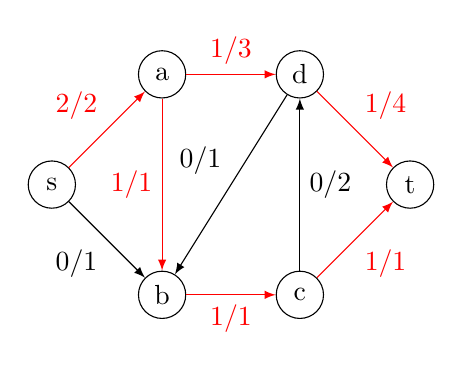
\begin{tikzpicture}[scale=0.7]
				\tikzset{noeud/.style={circle, draw=black, inner sep=0.1cm, minimum width=0.6cm}, fleche/.style={>=latex, ->}};
				\node[noeud] (s) at (0,0) {s};
				\node[noeud] (a) at (2, 2) {a};
				\node[noeud] (b) at (2, -2) {b};
				\node[noeud] (c) at (4.5, -2) {c};
				\node[noeud] (d) at (4.5, 2) {d};
				\node[noeud] (t) at (6.5,0) {t};

				\draw[fleche, red] (s) -- node[above left, red] {$2/2$}(a);
				\draw[fleche] (s) -- node[below left] {$0/1$}(b);
				\draw[fleche, red] (a) -- node[left,red] {$1/1$}(b);
				\draw[fleche, red] (a) -- node[above, red] {$1/3$}(d);
				\draw[fleche] (d) -- node[above left] {$0/1$}(b);
				\draw[fleche, red] (b) -- node[below, red] {$1/1$}(c);
				\draw[fleche, red] (d) -- node[above right, red] {$1/4$}(t);
				\draw[fleche, red] (c) -- node[below right, red] {$1/1$}(t);
				\draw[fleche] (c) -- node[right] {$0/2$}(d);
			\end{tikzpicture}
			\caption{Un exemple de flot}
		\end{figure}
	\end{minipage} \hfill
	\begin{minipage}[c]{0.45\linewidth}
		\begin{figure}
			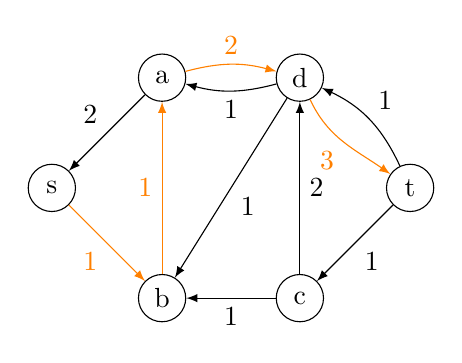
\begin{tikzpicture}[scale=0.7]
				\tikzset{noeud/.style={circle, draw=black, inner sep=0.1cm, minimum width=0.6cm}, fleche/.style={>=latex, ->}};
				\node[noeud] (s) at (0,0) {s};
				\node[noeud] (a) at (2, 2) {a};
				\node[noeud] (b) at (2, -2) {b};
				\node[noeud] (c) at (4.5, -2) {c};
				\node[noeud] (d) at (4.5, 2) {d};
				\node[noeud] (t) at (6.5,0) {t};

				\draw[fleche] (a) -- node[above left] {$2$}(s);
				\draw[fleche, orange] (s) -- node[below left, orange] {$1$}(b);
				\draw[fleche, orange] (b) -- node[left, orange] {$1$}(a);
				\draw[fleche, orange] (a) to[out=15, in=165]  node[above, orange] {$2$}(d);
				\draw[fleche] (d) to[out=195, in=345]  node[below] {$1$}(a);
				\draw[fleche] (d) -- node[below right] {$1$}(b);
				\draw[fleche] (c) -- node[below] {$1$}(b);
				\draw[fleche, orange] (d) to[out=295, in=145] node[below left, orange] {$3$}(t);
				\draw[fleche] (t) to[out=115, in=335] node[above right] {$1$}(d);
				\draw[fleche] (t) -- node[below right] {$1$}(c);
				\draw[fleche] (c) -- node[right] {$2$}(d);
			\end{tikzpicture}
			\caption{Le réseau résiduel associé}
		\end{figure}
	\end{minipage}
\end{frame}

\begin{frame}{Le réseau résiduel}
	Donc une augmentation possible du flot : \vfill
	\begin{minipage}[c]{0.45\linewidth}
		\begin{figure}
			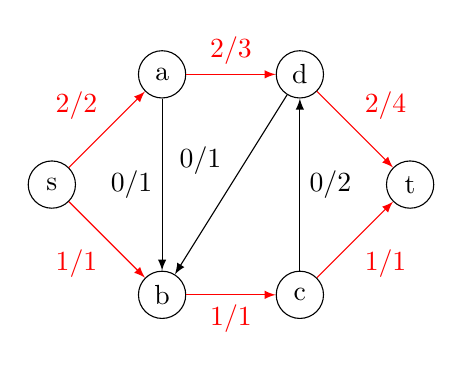
\begin{tikzpicture}[scale=0.7]
				\tikzset{noeud/.style={circle, draw=black, inner sep=0.1cm, minimum width=0.6cm}, fleche/.style={>=latex, ->}};
				\node[noeud] (s) at (0,0) {s};
				\node[noeud] (a) at (2, 2) {a};
				\node[noeud] (b) at (2, -2) {b};
				\node[noeud] (c) at (4.5, -2) {c};
				\node[noeud] (d) at (4.5, 2) {d};
				\node[noeud] (t) at (6.5,0) {t};

				\draw[fleche, red] (s) -- node[above left, red] {$2/2$}(a);
				\draw[fleche, red] (s) -- node[below left, red] {$1/1$}(b);
				\draw[fleche] (a) -- node[left] {$0/1$}(b);
				\draw[fleche, red] (a) -- node[above, red] {$2/3$}(d);
				\draw[fleche] (d) -- node[above left] {$0/1$}(b);
				\draw[fleche, red] (b) -- node[below, red] {$1/1$}(c);
				\draw[fleche, red] (d) -- node[above right, red] {$2/4$}(t);
				\draw[fleche, red] (c) -- node[below right, red] {$1/1$}(t);
				\draw[fleche] (c) -- node[right] {$0/2$}(d);
			\end{tikzpicture}
			\caption{Un exemple de flot}
		\end{figure}
	\end{minipage} \hfill
	\begin{minipage}[c]{0.45\linewidth}
		\begin{figure}
			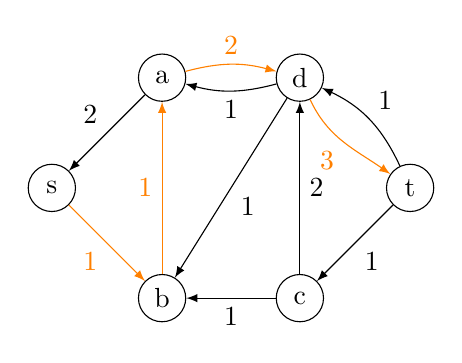
\begin{tikzpicture}[scale=0.7]
				\tikzset{noeud/.style={circle, draw=black, inner sep=0.1cm, minimum width=0.6cm}, fleche/.style={>=latex, ->}};
				\node[noeud] (s) at (0,0) {s};
				\node[noeud] (a) at (2, 2) {a};
				\node[noeud] (b) at (2, -2) {b};
				\node[noeud] (c) at (4.5, -2) {c};
				\node[noeud] (d) at (4.5, 2) {d};
				\node[noeud] (t) at (6.5,0) {t};

				\draw[fleche] (a) -- node[above left] {$2$}(s);
				\draw[fleche, orange] (s) -- node[below left, orange] {$1$}(b);
				\draw[fleche, orange] (b) -- node[left, orange] {$1$}(a);
				\draw[fleche, orange] (a) to[out=15, in=165]  node[above, orange] {$2$}(d);
				\draw[fleche] (d) to[out=195, in=345]  node[below] {$1$}(a);
				\draw[fleche] (d) -- node[below right] {$1$}(b);
				\draw[fleche] (c) -- node[below] {$1$}(b);
				\draw[fleche, orange] (d) to[out=295, in=145] node[below left, orange] {$3$}(t);
				\draw[fleche] (t) to[out=115, in=335] node[above right] {$1$}(d);
				\draw[fleche] (t) -- node[below right] {$1$}(c);
				\draw[fleche] (c) -- node[right] {$2$}(d);
			\end{tikzpicture}
			\caption{Le réseau résiduel associé}
		\end{figure}
	\end{minipage}
\end{frame}

\begin{frame}{Les algorithmes}
	Varient sur le choix des chaînes améliorantes : \vfill
\end{frame}

\begin{frame}{Les algorithmes}
	Varient sur le choix des chaînes améliorantes : \vfill
	\begin{itemize}
		\item \underline{Ford-Fulkerson} : choix aléatoire \vfill
	\end{itemize}
\end{frame}

\begin{frame}{Les algorithmes}
	Varient sur le choix des chaînes améliorantes : \vfill
	\begin{itemize}
		\item \underline{Ford-Fulkerson} : choix aléatoire \vfill
		\item \underline{Edmonds-Karp} : la plus petite chaîne en nombre d'arcs\vfill
	\end{itemize}
\end{frame}

\begin{frame}{Les algorithmes}
	Varient sur le choix des chaînes améliorantes : \vfill
	\begin{itemize}
		\item \underline{Ford-Fulkerson} : choix aléatoire \vfill
		\item \underline{Edmonds-Karp} : la plus petite chaîne en nombre d'arcs\vfill
		\item \underline{Dinic} : l'ensemble des plus petites chaînes en nombre d'arcs \vfill
	\end{itemize}
\end{frame}

\begin{frame}{Les limites de ces algorithmes}
	Considérons le graphe suivant :\vfill

	\begin{figure}
	\begin{center}
	\scalebox{0.6}{
		\begin{tikzpicture}
			\tikzset{noeud/.style={circle, draw=black, text centered,minimum size=26pt, inner sep=0pt},
			fleche/.style={thick}};

			\node[noeud] (t) at (14, 0) {$t$};
			\node[noeud] (s) at (2, 0) {$s$};

			\foreach \x in {2, 3, 4, 5}{
				\node[noeud] (\x) at (2*\x, 0) {$\x$}; 
			}

			\foreach \y/\ytext in {3.5/6, 1.7/7, -1.7/n-1, -3.5/n}{
				\node[noeud] (\ytext) at (12, \y) {$\ytext$};
				\draw[fleche] (5) --node[right] {$1$} (\ytext) --node[left] {$1$} (t);
			}

			\node (point) at (12, 0) {$\vdots$};

			\draw[fleche] (s) --node[above] {$\infty$} (2) --node[above] {$\infty$} (3) --node[above] {$\infty$}
			(4) --node[above] {$\infty$} (5) ;

		\end{tikzpicture}}
	\end{center}
\end{figure} \vfill
\end{frame}

\begin{frame}{Introduction aux opérations}
	Considérons le graphe suivant :\vfill

	\begin{figure}
	\begin{center}
	\scalebox{0.6}{
		\begin{tikzpicture}
			\tikzset{noeud/.style={circle, draw=black, text centered,minimum size=26pt, inner sep=0pt},
			fleche/.style={thick}};

			\node[noeud] (t) at (14, 0) {$t$};
			\node[noeud] (s) at (2, 0) {$s$};

			\foreach \x in {2, 3, 4, 5}{
				\node[noeud] (\x) at (2*\x, 0) {$\x$}; 
			}

			\foreach \y/\ytext in {3.5/6, 1.7/7, -1.7/n-1, -3.5/n}{
				\node[noeud] (\ytext) at (12, \y) {$\ytext$};
				\draw[fleche] (5) --node[right] {$1$} (\ytext) --node[left] {$1$} (t);
			}

			\node (point) at (12, 0) {$\vdots$};

			\draw[fleche] (s) --node[above] {$\infty$} (2) --node[above] {$\infty$} (3) --node[above] {$\infty$}
			(4) --node[above] {$\infty$} (5) ;

		\end{tikzpicture}}
	\end{center}
\end{figure} \vfill
\begin{alertblock}{Constat}
Il met en défaut les algorithmes de recherche de chaînes améliorantes.
\end{alertblock}
\end{frame}

\begin{frame}{Introduction aux opérations}
	Considérons le graphe suivant :\vfill

	\begin{figure}
	\begin{center}
	\scalebox{0.6}{
		\begin{tikzpicture}
			\tikzset{noeud/.style={circle, draw=black, text centered,minimum size=26pt, inner sep=0pt},
			fleche/.style={thick}};

			\node[noeud] (t) at (14, 0) {$t$};
			\node[noeud] (s) at (2, 0) {$s$};

			\foreach \x in {2, 3, 4, 5}{
				\node[noeud] (\x) at (2*\x, 0) {$\x$}; 
			}

			\foreach \y/\ytext in {3.5/6, 1.7/7, -1.7/n-1, -3.5/n}{
				\node[noeud] (\ytext) at (12, \y) {$\ytext$};
				\draw[fleche] (5) --node[right] {$1$} (\ytext) --node[left] {$1$} (t);
			}

			\node (point) at (12, 0) {$\vdots$};

			\draw[fleche] (s) --node[above] {$\infty$} (2) --node[above] {$\infty$} (3) --node[above] {$\infty$}
			(4) --node[above] {$\infty$} (5) ;

		\end{tikzpicture}}
	\end{center}
\end{figure} \vfill
\begin{exampleblock}{Intuition}
Agir de façon locale au noeud $5$, afin d'envoyer du flot à tous ses voisins en une seule opération.
\end{exampleblock}
\end{frame}



